\documentclass[12pt,pdf,utf8,ukrainian,aspectratio=169]{beamer}
\usepackage[T2A]{fontenc}
\usepackage[utf8]{inputenc}
%\usepackage[ukrainian,english]{babel}
%\usepackage{hyphenat}
%\usepackage{amsfonts}
%\usepackage{polyglossia}
%\usepackage{mathptmx}

\usepackage{nameref}
\makeatletter
\newcommand*{\currentname}{\@currentlabelname}

\renewcommand{\sfdefault}{fds}\normalfont


\usetheme{AnnArbor}
\usecolortheme{crane}

\setbeamertemplate{navigation symbols}{}
\setbeamercolor{frametitle}{fg=black,bg=white}
\setbeamercolor{title}{fg=black,bg=yellow!85!orange}

\beamersetuncovermixins{\opaqueness<1>{25}}{\opaqueness<2->{15}}
\begin{document}
	\title[Коментарі etc.]{
		Коментарі, документація, \newline 
		а також все що з цим пов'язане \newline 
		і зможе зробити наш код ще кращим
	}
	\author{Назар Герасимчук}
	\date{\today} 
	
	\begin{frame}
		\titlepage
	\end{frame}
	
%	\begin{frame}\frametitle{Зміст}
%		\tableofcontents
%	\end{frame} 

	\section{Що і до чого?}
	\begin{frame}\frametitle{\currentname} 
		\begin{block}
		{\LARGE Не коментуйте поганий код -- \\ перепишіть його.} 
			\begin{flushright}
				Б.~Керніган і П.~Плауер
			\end{flushright}
		\end{block}		
		\begin{itemize}
			\item \textbf{Найкраща допомога} розробнику -- хороший коментар в коді. \pause
			\item \textbf{Найбільше засмічують} код беззмістовні коментарі. \pause
			\item \textbf{Найбільшу шкоду} приносить коментар який втратив свою актуальність (хибний, дезінформативний).
		\end{itemize}
	\end{frame}

	\section{Філософський погляд на коментарі}
	\begin{frame}\frametitle{\currentname} 
		\begin{block}
			{\LARGE Насправді коментарі -- \\ неуникне зло.}
		\end{block}	
		
		\begin{itemize}
			\item Мови програмування недостатньо виразні. \pause
			\item Програмування -- процес невдалого виразу власних думок. \pause
			\item Коментарі -- ознака невдачі. Гордитися тут нічим.
		\end{itemize}
	\end{frame}

	\section{Приклад до обговорення} 
	\begin{frame}\frametitle{\currentname}
		\begin{figure}
			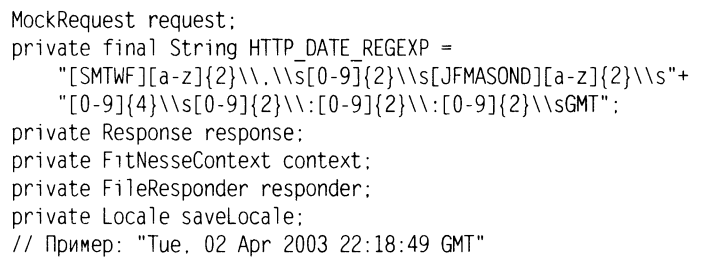
\includegraphics[scale=0.8]{clean_code_1.png} 
			\newline \newline
			\textit{Що сталося з коментарем і з тією стрічкою яку він повинен був описувати?}
		\end{figure}
	\end{frame}

	\section{Коментарі не компенсують поганого коду}
	\begin{frame}\frametitle{\currentname} 
		\begin{block}
			{\Large Ви пишете модуль, і розумієте що він не\-кон\-тро\-льо\-ва\-но розрісся, 
				став дуже заплутаним. Тут, згадуєте цю презентацію\footnote{ну як вам рекурсія?} 
				і думаєте \textit{<<A давай-но я зараз понаписую коментарів, щоб код був зрозуміліший>>}. \\ 
				\textbf{Ні! Так не буде краще. Потрібно переписати код модуля!}
			}
		\end{block}	
	\end{frame}
	
	\section{Пояснюйте \textbf{що} ви робите в коді}
	\begin{frame}\frametitle{\currentname}
			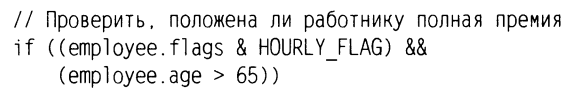
\includegraphics[scale=0.8]{clean_code_2_1.png}\hfill	
			\vfill	
			\noindent\rule{\textwidth}{1pt}
			\vfill
			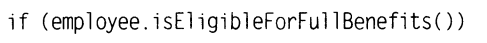
\includegraphics[scale=0.8]{clean_code_2_2.png}\hfill
	\end{frame}
	
	\section{Корисні коментарі}
	\subsection{Юридичні нотації}
	\begin{frame}\frametitle{\currentname}
		\begin{center}
			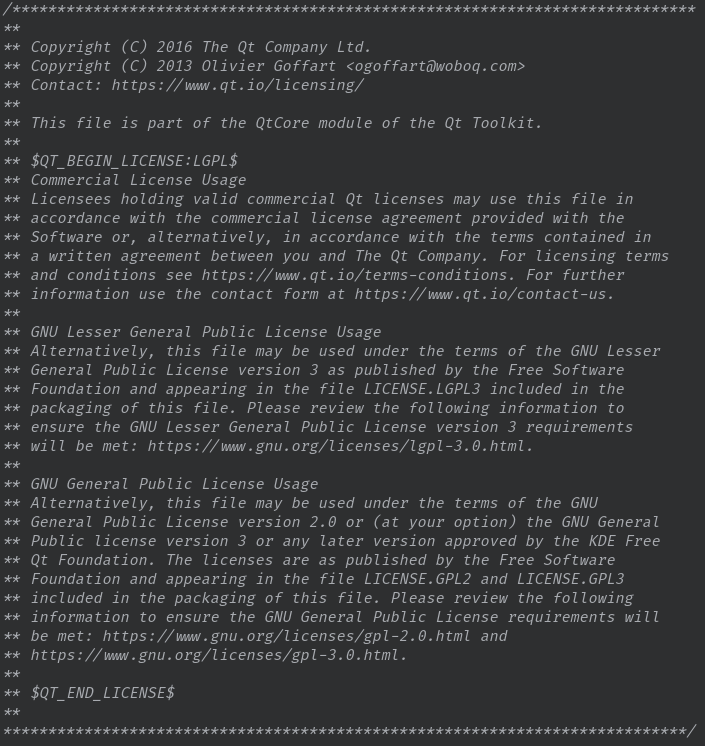
\includegraphics[scale=0.35]{clean_code_3_1.png}
		\end{center}
	\end{frame}
	
	\begin{frame}\frametitle{\currentname}
		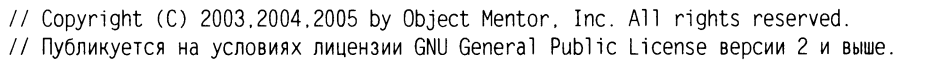
\includegraphics[scale=0.65]{clean_code_3.png}\hfill	
	\end{frame}
	
	\subsection{Інформативні коментарі}
	\begin{frame}\frametitle{\currentname}
		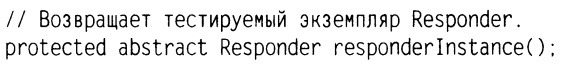
\includegraphics[scale=0.8]{clean_code_4_1.png}
		\footnote{Хіба не краще перейменувати метод?}
		\hfill	
		\vfill	
		\noindent\rule{\textwidth}{1pt}
		\vfill
		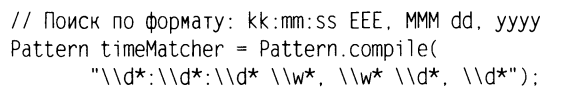
\includegraphics[scale=0.8]{clean_code_4_2.png}
		\footnote{Хіба не краще винести в спеціальний клас, що перетворює формати дати і часу?}
		\hfill
	\end{frame}

	\subsection{Пояснення намірів}
	\begin{frame}\frametitle{\currentname}
		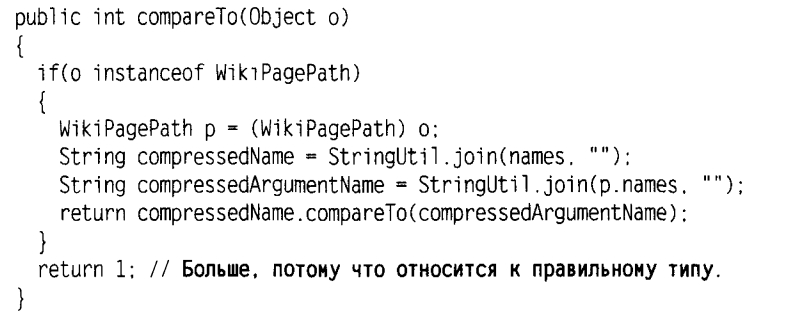
\includegraphics[scale=0.65]{clean_code_5_1.png}
		\footnote{Автор вирішив, що при порівнянні двох об'єктів об'єкти його класу повинні 
			знаходитися в порядку сортування вище, чим об'єкти будь-якого іншого класу.}
		\hfill	
	\end{frame}
	
	\begin{frame}\frametitle{\currentname}
		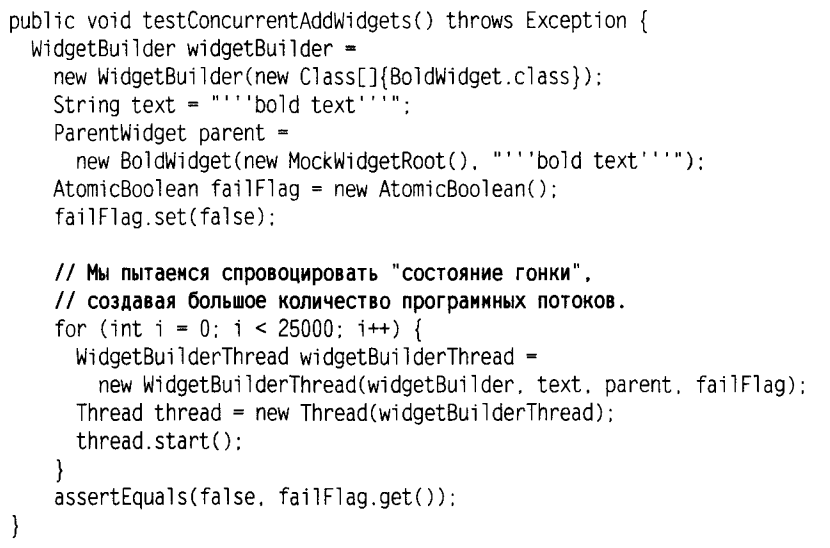
\includegraphics[scale=0.4]{clean_code_5_2.png}
		\footnote{Можна не погодитися з тим як автор вирішує проблему, проте в крайньому разі ви знаєте що саме автор намагається зробити.}
		\hfill	
	\end{frame}

	\subsection{Пояснення}
	\begin{frame}\frametitle{\currentname}
		\begin{columns}
			\begin{column}{7cm}
				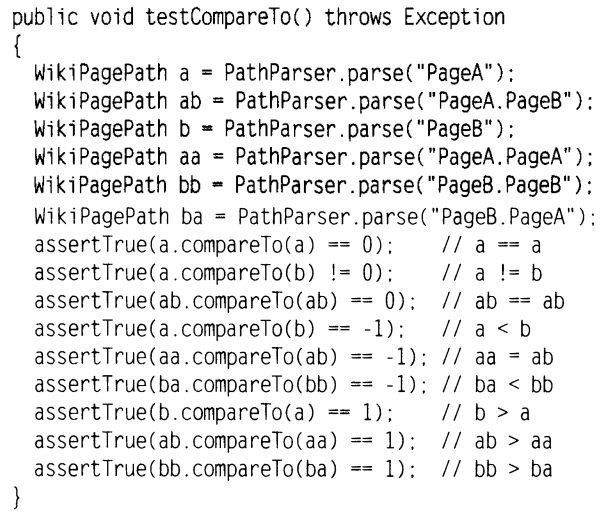
\includegraphics[scale=0.45]{clean_code_6.png}
			\end{column}
			\begin{column}{5cm} 
				\small
				Пояснення загадкового аргументу, або значення що повертається. Загалом варто обдумати як краще це \textit{зобразити} засобами мови програмування. \\
				Хоча часто подібна ситуація трапляється коли ви працюєте з готовою бібліотекою чи модулем.
			\end{column}
		\end{columns}	
	\end{frame}

	\subsection{Пояснення і ризики}
	\begin{frame}\frametitle{\currentname}
	\begin{columns}
		\begin{column}{7cm}
			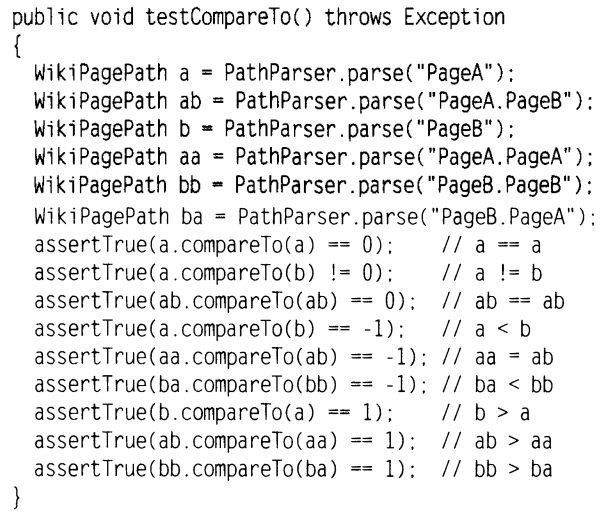
\includegraphics[scale=0.45]{clean_code_6.png}
		\end{column}
		\begin{column}{5cm} 
			\small
			Виникає ризик що коментар буде неправильним. Це справді важко перевірити, самі переконайтеся.
		\end{column}
	\end{columns}	
	\end{frame}

	\subsection{Попередження про можливі наслідки}
	\begin{frame}\frametitle{\currentname}
		\begin{columns}
			\begin{column}{8cm}
				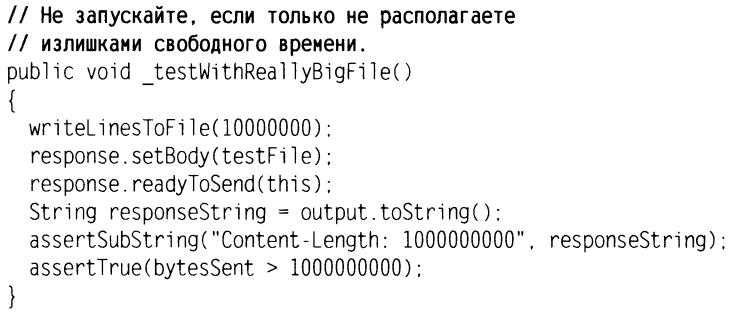
\includegraphics[scale=0.45]{clean_code_7.png}
			\end{column}
			\begin{column}{5cm} 
				\small
				Можливо не найкраще рішення, але тут все зрозуміло з цим тестом.
			\end{column}
		\end{columns}	
	\end{frame}

	\begin{frame}\frametitle{\currentname}
		\begin{columns}
			\begin{column}{10cm}
				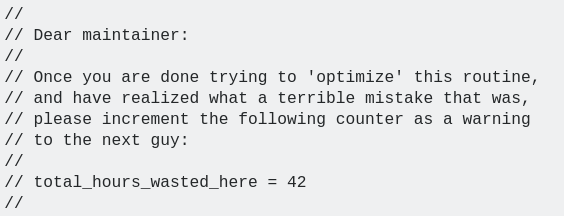
\includegraphics[scale=0.65]{Comment_02.png}
			\end{column}
			\begin{column}{5cm} 
				\small
				Хрестоматійний приклад.
			\end{column}
		\end{columns}	
	\end{frame}
	
	\begin{frame}\frametitle{\currentname}
		\Large
		Можливо це не найкращі коментарі, проте, їх наявність точно відіб'є бажання		
		у типового програміста витрачати робочий час на щось інше, крім як на вирішення
		своїх прямих задач.
	\end{frame}

	\subsection{Коментарі \texttt{TODO}}
	\begin{frame}\frametitle{\currentname}
		\begin{columns}
			\begin{column}{7cm}
				
\includegraphics[scale=0.5]{clean_code_8.png}
			\end{column}
			\begin{column}{5cm} 
				\small
				\begin{itemize}
					\item Чого ф-ія не реалізована? 
					\item Реалізувати потрібно, проте \textit{чомусь} не зараз.
					\item Залежність?
					\item Функції в IDE.
				\end{itemize}
			\end{column}
		\end{columns}		
	\end{frame}

	\begin{frame}\frametitle{\currentname}
		
\includegraphics[scale=0.65]{Comment_06.png}
		\footnote{Тяжко жити, шкода вмерти. Не всі \texttt{TODO}-коментарі корисні.}
		\hfill
	\end{frame}

	\section{Погані коментарі}
	\begin{frame}\frametitle{\currentname}
		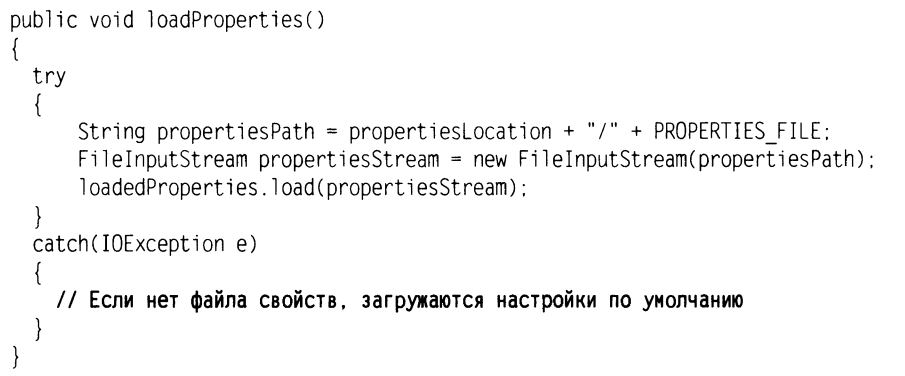
\includegraphics[scale=0.5]{clean_code_9.png}
		\footnote{Що означає коментар? Хто цим буде займатися? Чого добивався автор? Чи може це такий \texttt{TODO}-коментар?}
		\hfill
	\end{frame}	
	
	\subsection{Надлишкові коментарі}
	\begin{frame}[label={slideError}]\frametitle{\currentname}
		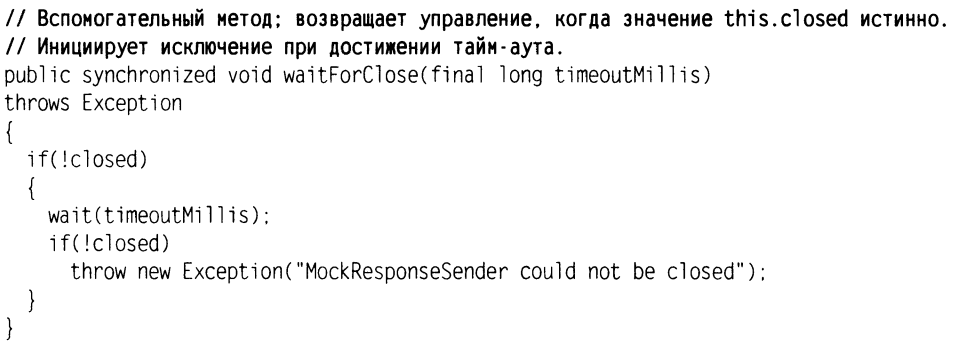
\includegraphics[scale=0.5]{clean_code_10.png}
		\footnote{Коментар читається не простіше ніж сам код. Коментар є неточним і нав'язує читачу певні ідеї які можуть бути відмінні від того що декларується в коді.}
		\hfill
	\end{frame}	

	\begin{frame}\frametitle{\currentname}
		\begin{columns}
			\begin{column}{7cm}
				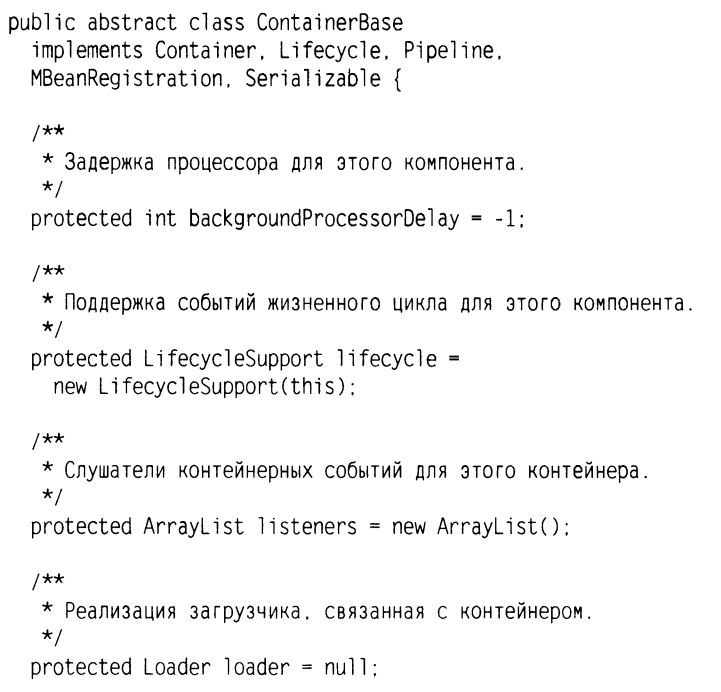
\includegraphics[scale=0.35]{clean_code_11_1.png}
			\end{column}
			\begin{column}{7cm} 
				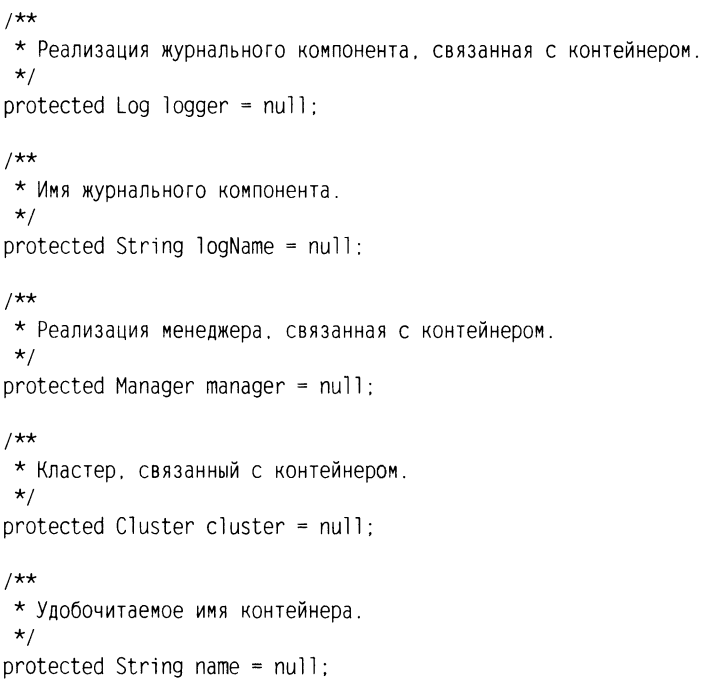
\includegraphics[scale=0.35]{clean_code_11_2.png}
			\end{column}
		\end{columns}	
	\end{frame}	

	\subsection{Недостовірні коментарі}
	\begin{frame}\frametitle{\currentname}
		\begin{columns}
			\begin{column}{8cm}
				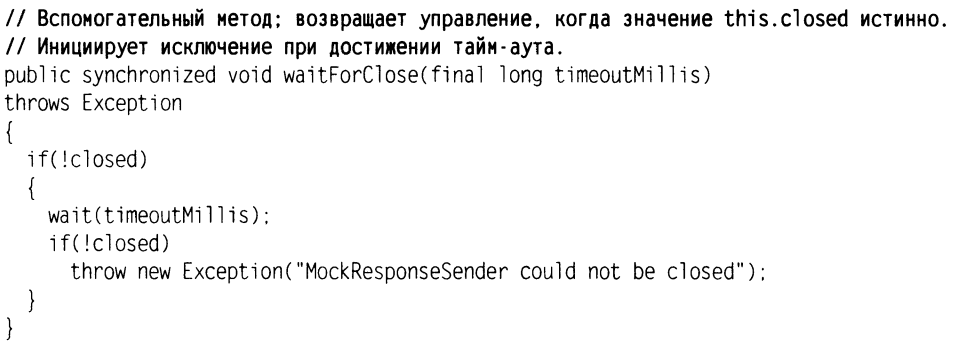
\includegraphics[scale=0.3]{clean_code_10.png}
			\end{column}
			\begin{column}{7cm} 
				\small
				\begin{itemize}
					\item Код зі слайду~\ref{slideError}. \pause
					\item Метод \textbf{не} повертає керування \textbf{коли} \texttt{this.closed} стає істинним. \pause
					\item Метод повертає керування \textbf{якщо} \texttt{this.closed} істинне, інакше, чекає таймауту і генерує виключення у випадку якщо \texttt{this.closed} так і не стало істинне. \pause
					\item Проблеми будуть не в того хто це написав, а в того хто унаслідує цей код.
				\end{itemize}
			\end{column}
		\end{columns}	
	\end{frame}	
	
	
	\subsection{Журнальні коментарі}
	\begin{frame}[label={slideError}]\frametitle{\currentname}
		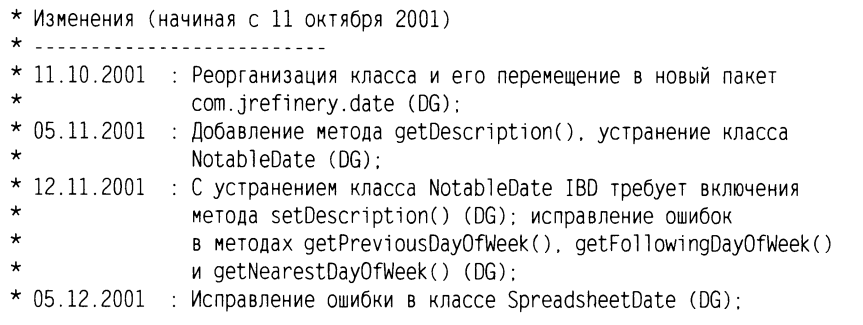
\includegraphics[scale=0.5]{clean_code_12.png}
		\footnote{З моменту коли почали використовувати системи контролю версій коду -- про подібні речі треба одразу ж забувати.}
		\hfill
	\end{frame}	

	\subsection{Шум}
	\begin{frame}[label={slideError}]\frametitle{\currentname}
		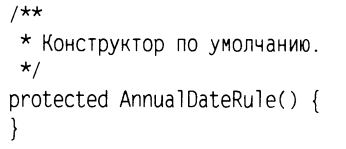
\includegraphics[scale=0.5]{clean_code_13_1.png} \\
		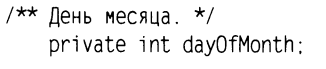
\includegraphics[scale=0.5]{clean_code_13_2.png} \\
		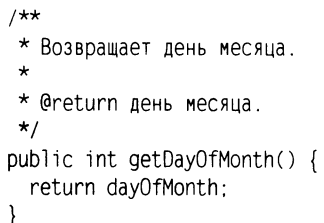
\includegraphics[scale=0.5]{clean_code_13_3.png} \\
	\end{frame}	

	\subsection{Шум}
	\begin{frame}[label={slideError}]\frametitle{\currentname}
		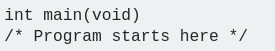
\includegraphics[scale=0.7]{Comment_05.png}
	\end{frame}	

	\subsection{Небезпечний шум}

	\begin{frame}\frametitle{\currentname}
		\begin{columns}
			\begin{column}{8cm}
				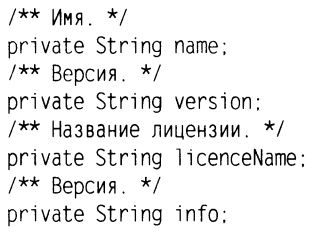
\includegraphics[scale=0.7]{clean_code_15.png}
			\end{column}
			\begin{column}{7cm} 
				\footnotesize
				\begin{itemize}
					\item Яка користь з коментарів такого типу? \pause
					\item Це шумові коментарі, викликані бажанням когось покоментувати.\pause
					\item Перечитайте уважніше. \pause
					\item Знайшли помилку? \pause
					\item Ctrl+C + Ctrl+V
					\item Якщо автори не слідкують за коментарями в момент написання, то як можна очікувати що такі коментарі принесуть користь читачам?
				\end{itemize}
			\end{column}
		\end{columns}	
	\end{frame}	

	\begin{frame}\frametitle{\currentname}
		\begin{columns}
			\begin{column}{6cm}
				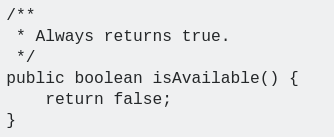
\includegraphics[scale=0.7]{Comment_07.png}
			\end{column}
			\begin{column}{8cm} 
				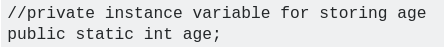
\includegraphics[scale=0.7]{Comment_03.png}
			\end{column}
		\end{columns}	
	\end{frame}	

	\subsection{Коментар чи функція?}
	\begin{frame}\frametitle{\currentname}
		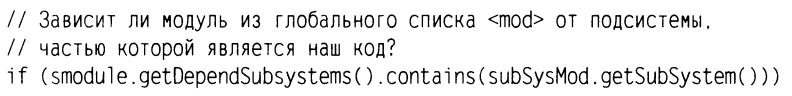
\includegraphics[scale=0.6]{clean_code_16.png}
		\footnote{Імовірно програміст спершу написав коментар, потім по коментару написав відповідний код. Але він забув переглянути написаний код...}
		\hfill	
		\vfill	
		\noindent\rule{\textwidth}{1pt}
		\vfill
		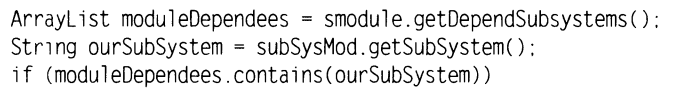
\includegraphics[scale=0.6]{clean_code_16_1.png}
		\hfill
	\end{frame}

	\subsection{Закоментований код}
	\begin{frame}\frametitle{\currentname}
		\begin{block}
			{\LARGE В програмуванні навряд чи трапиться звичка більш огидна як залишений закоментований код. }
		\end{block}
		\begin{itemize}
			\item Іншим програмістам не вистачить хоробрості його видалити.
			\item Чи важливі закоментовані стрічки?
			\item Може це просто \textit{мотлох}?
			\item Забули про систему контролю версій?
		\end{itemize}
	\end{frame}

	\subsection{Нелокальна інформація}
	\begin{frame}\frametitle{\currentname}
		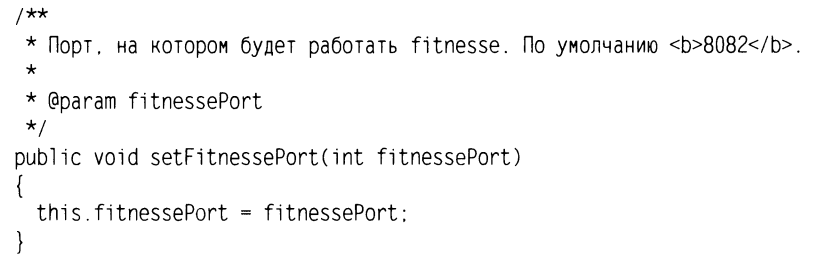
\includegraphics[scale=0.6]{clean_code_17.png}
		\footnote{Хто прослідкує за зміною порта по замовчуванню?}
		\hfill	
	\end{frame}

	\subsection{Неочевидні коментарі}
	\begin{frame}\frametitle{\currentname}
		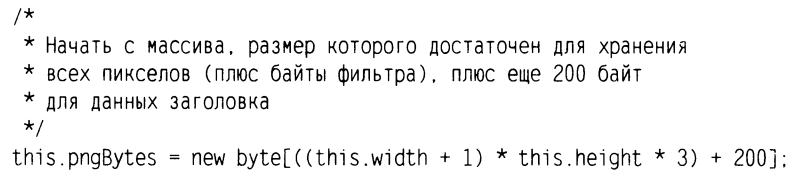
\includegraphics[scale=0.6]{clean_code_18.png}
		\footnote{Що таке байти фільтра? Як вони пов'язані з \texttt{+1}?
		Або з \texttt{*3}? Один піксель відповідає одному байту? Чого 200?..}
		\hfill	
	\end{frame}

	\section{Цікаві коментарі в історії}
	\begin{frame}\frametitle{\currentname}
	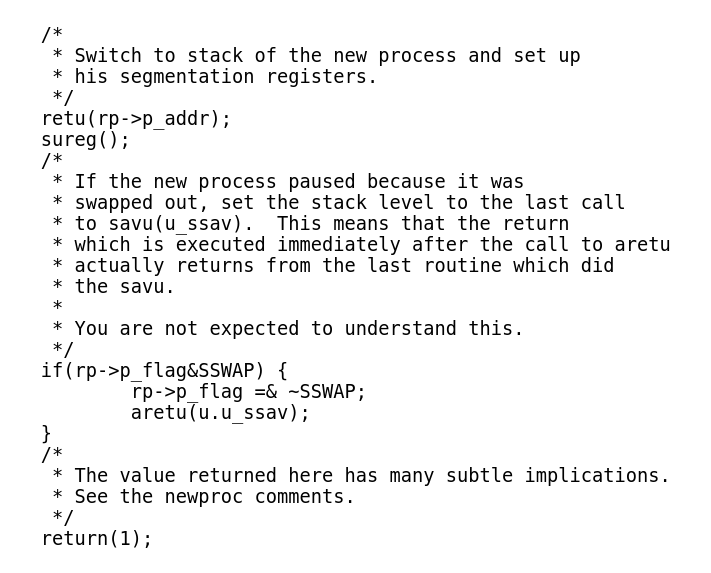
\includegraphics[scale=0.6]{DMR_01.png}
	\end{frame}
	
	\begin{frame}\frametitle{\currentname}
		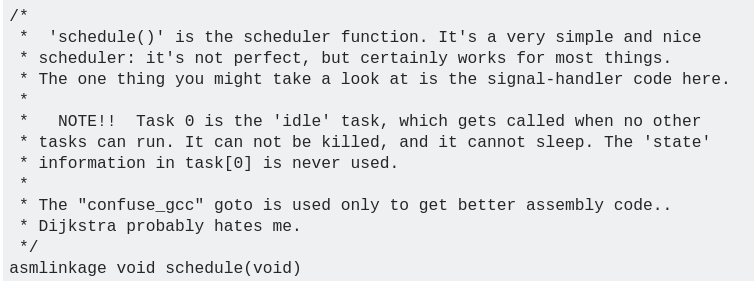
\includegraphics[scale=0.6]{Dij.png}
	\end{frame}

	\section{Практична частина}
	\begin{frame}\frametitle{\currentname}
		
	\end{frame}

	\begin{frame}[allowframebreaks]
		\frametitle<presentation>{Джерела}    
		\begin{thebibliography}{10}    
			\setbeamertemplate{bibliography item}[book]
			\bibitem{CleanCode}
			Robert~C. Martin.
			\newblock {\em Clean Code - a Handbook of Agile Software Craftsmanship}.
			\newblock Prentice Hall, 2009.
			
			\bibitem{Ker}
			B.~W.~Kernighan and P.~J.~Plauge
			\newblock {\em The Elements of Programming Style}.
			\newblock New~York, 1978.
			
			\setbeamertemplate{bibliography item}[online]	
			\bibitem{DMR}
			Dennis Ritchie.
			\newblock {\em Odd Comments and Strange Doings in Unix}.
%			\newblock {\tiny Нажаль, з веб-архіва. Так як чомусь bell-labs після смерті Деніса Річі вирішила не хостити його записки.}
			\newblock http://web.archive.org/web/20040206202840/http://cm.bell-labs.com/cm/cs/who/dmr/odd.html
			
			\setbeamertemplate{bibliography item}[online]
			\bibitem{GovnoKod}
			Говнокод.ру	
			\newblock <<По колено в коде>> https://www.govnokod.ru/
		\end{thebibliography}
	\end{frame}	
\end{document}